% Sample Dissertation, Thesis, or Document %
%            for use with the              %
%  University of Arizona Thesis Class,     %
%               uathesis.cls               %
%------------------------------------------%

% We'll use the uathesis document class (duh).  The uncommented line
% below will produce a Dissertation, the others would produce a Thesis
% or a Document.  There are other options available to you like turning
% on the copyright statement and replacing the year on the title page
% with a "generated on" stamp (handy for early drafts).  To find out
% what the available options are, take a look into the uathesis.cls
% file and look for the \DeclareOption commands near the top of that
% file.
% There are five copyright options.  Copyright, no copyright, and three
% different Creative Commons licences.  Use the one you want (If you go
% Creative Commons, I (DM) think the CC-BY-ND makes the most sense)  See
% uathesis.cls for the reason why the non-commercial licenses are not
% included.
%\documentclass[dissertation]{uathesis}
\documentclass[dissertation,copyright]{uathesis}
%\documentclass[dissertation,CC-BY]{uathesis}
%\documentclass[dissertation,CC-BY-SA]{uathesis}
%\documentclass[dissertation,CC-BY-ND]{uathesis}
%\documentclass[thesis]{uathesis}
%\documentclass[document]{uathesis}

%\usepackage{setspace}
%\doublespacing
% or:
%\singlespacing


% Package Usage
% These are the packages that we need
\usepackage{graphicx}
\usepackage{natbib}			% natbib is available on most systems, and is
					% terribly handy.
					% If you want to use a different Bibliography package, 
					% you should be able to, just change this
					% and the \bibliographystyle command below.  Be warned
					% that you may need to do a little hacking to get
					% the REFERENCES item to show up in your TOC.
\usepackage{graphicx}
\usepackage[caption=false,font=footnotesize,labelfont=sf,textfont=sf]{subfig}
\usepackage[cmex10]{amsmath}
\usepackage{latexsym}
\usepackage{amssymb}
% Compatibility with the AASTEX package 
% of the American Astronomical Society.
%\usepackage{deluxetable}		% Allows use of AASTEX deluxe tables
%\usepackage{aastex_hack}		% Allows other AASTEX functionality.

% These are other packages that you might find useful.
% For controlling the fonts, see
% http://www.math.uiuc.edu/~hartke/computer/latex/survey/survey.html
% The following is a nice font set:
%\usepackage{mathtime}			% Times for letters; Belleek math.
%
\usepackage{amsmath}			% AMS Math (advanced math typesetting)
\usepackage{lscape}			% Used for making fitting large tables in by putting them landscape
\usepackage{refs}	
%
% If you are using hyper-ref (recommended), this command must go after all 
% other package inclusions (from the hyperref package documentation).
% The purpose of hyperref is to make the PDF created extensively
% cross-referenced.
%\usepackage[dvips,bookmarks,colorlinks=true,urlcolor=black,linkcolor=black,citecolor=black]{hyperref}
\usepackage[bookmarks,colorlinks=true,urlcolor=black,linkcolor=black,citecolor=black]{hyperref}

\usepackage{rotating}
\usepackage{multirow,tabularx}

% Set up some values.
\completetitle{Parameter Advising for Multiple Sequence Alignment}
\pagetitle{Parameter Advising for}{Multiple Sequence Alignment}{}
%\completetitle{Constructing advisors for multiple sequence alignment}
%\completetitle{Multiple Sequence Alignment Accuracy Improvement Through Advising and Realignment.}
\fullname{Daniel Frank DeBlasio}			% Grad college wants your full name here.
\degreename{Doctor of Philosophy}	% Title of your degree.



\newcommand{\argmin}{\mathop{\mathrm{argmin}}}
\newcommand{\argmax}{\mathop{\mathrm{argmax}}}

\DeclareTextFontCommand{\emph}{\em\bfseries}


%estimators
\newcommand{\Facet}{\texttt{Facet}}
\newcommand{\Mos}{\texttt{MOS}}
\newcommand{\Coffee}{\texttt{COFFEE}}
\newcommand{\Glpk}{\texttt{GLPK}}
\newcommand{\Normd}{\texttt{NorMD}}
\newcommand{\Altwoco}{\texttt{AL2CO}}
\newcommand{\Predsp}{\texttt{PredSP}}
\newcommand{\Hot}{\texttt{HoT}}
\newcommand{\Guidance}{\texttt{GUIDANCE}}
\newcommand{\Psar}{\texttt{PSAR}}
\newcommand{\Rascal}{\texttt{RASCAL}}
\newcommand{\Aqua}{\texttt{AQUA}}
\newcommand{\Leon}{\texttt{LEON}}
\newcommand{\Pacalci}{\texttt{PAcAlCI}}
\newcommand{\Glprobs}{\texttt{GLProbs}}
\newcommand{\Fsm}{\texttt{FSM}}
\newcommand{\Lssvm}{\texttt{LS-SVM}}
\newcommand{\Alexsys}{\texttt{AlexSys}}
\newcommand{\Crumble}{\texttt{Crumble}}
\newcommand{\Prune}{\texttt{Prune}}
\newcommand{\Irmsd}{\texttt{iRMSD}}
\newcommand{\Strike}{\texttt{STRIKE}}
\newcommand{\Aliscore}{\texttt{ALISCORE}}
\newcommand{\Statsigma}{\texttt{StatSigMa}}
\newcommand{\Gblocks}{\texttt{GBLOCKS}}
\newcommand{\Tcs}{\texttt{TCS}}
\newcommand{\Zorro}{\texttt{ZORRO}}

%aligners
\newcommand{\Opal}{\texttt{Opal}}
\newcommand{\Clustal}{\texttt{Clustal}}
\newcommand{\Tcoffee}{\texttt{T-Coffee}}
\newcommand{\Muscle}{\texttt{Muscle}}
\newcommand{\Mafft}{\texttt{MAFFT}}
\newcommand{\Probcons}{\texttt{ProbCons}}
\newcommand{\Multiclustal}{\texttt{MULTICLUSTAL}}
\newcommand{\Probalign}{\texttt{PROBALIGN}}
\newcommand{\Mummals}{\texttt{MUMMALS}}
\newcommand{\Mcoffee}{\texttt{M-Coffee}}
\newcommand{\Comalign}{\texttt{ComAlign}}
\newcommand{\Mergealign}{\texttt{MergeAlign}}
\newcommand{\Kalign}{\texttt{Kalign}}
\newcommand{\Promals}{\texttt{PROMALS}}
\newcommand{\Ispalign}{\texttt{ISPalign}}
\newcommand{\Dialign}{\texttt{\mbox{DIALIGN}}}
\newcommand{\Prank}{\texttt{PRANK}}
\newcommand{\Msaprobs}{\texttt{MSAProbs}}


%other tools
\newcommand{\Cplex}{\texttt{CPLEX}}
\newcommand{\Blast}{\texttt{BLAST}}
\newcommand{\Svmlight}{$\texttt{SVM}^\texttt{light}$}
\newcommand{\Pfam}{\texttt{PFam}}

%benchmarks
\newcommand{\Balibase}{\texttt{BAliBASE}}
\newcommand{\Pali}{\texttt{PALI}}
\newcommand{\Sabmark}{\texttt{SABmark}}
\newcommand{\Oxbench}{\texttt{OxBench}}
\newcommand{\Scop}{\texttt{SCOP}}
\newcommand{\Sabre}{\texttt{SABRE}}
\newcommand{\Bench}{\texttt{BENCH}}
\newcommand{\Prefab}{\texttt{PREFAB}}

%matricies
\newcommand{\Blosum}{\texttt{BLOSUM}}
\newcommand{\Blsm}{\texttt{BLSM}}
\newcommand{\Pam}{\texttt{PAM}}
\newcommand{\Vtml}{\texttt{VTML}}
\newcommand{\Psipred}{\texttt{PSIPRED}}

%features
\newcommand{\BL}{\texttt{BL}}
\newcommand{\SA}{\texttt{SA}}
\newcommand{\SI}{\texttt{SI}}
\newcommand{\GC}{\texttt{GC}}
\newcommand{\AI}{\texttt{AI}}
\newcommand{\SP}{\texttt{SP}}
\newcommand{\GP}{\texttt{GP}}
\newcommand{\AS}{\texttt{AS}}
\newcommand{\GE}{\texttt{GE}}
\newcommand{\GO}{\texttt{GO}}
\newcommand{\IC}{\texttt{IC}}
\newcommand{\CC}{\texttt{CC}}


\newcommand{\Greedy}{\texttt{Greedy}}
\newcommand{\Java}{\texttt{Java}}

%%%%%%%%%%%%%%%%%%%%%%%%%%%%%%%%%%%%%%%%%
% From John's Header File For Formatting from JCB Paper




\newenvironment{List}[1]
 {\begin{list}{$\bullet$}{
  \settowidth{\labelwidth}{\rm #1}
  \renewcommand{\makelabel}{\hfil\rm}
  \setlength{\itemsep}{0ex}
  \setlength{\parsep}{0ex}
  \setlength{\partopsep}{0ex}
  \setlength{\parskip}{0ex}
  \setlength{\topsep}{1.25ex}
  \setlength{\listparindent}{\parindent}
  \setlength{\leftmargin}{\parindent}
  \advance\leftmargin\labelwidth
  \advance\leftmargin\labelsep
  \setlength{\rightmargin}{\parindent}
 }}{\end{list}}

\newenvironment{SpacedList}[1]
 {\begin{list}{$\bullet$}{
  \settowidth{\labelwidth}{\rm #1}
  \renewcommand{\makelabel}{\hfil\rm}
  \setlength{\itemsep}{1.25ex}
  \setlength{\parsep}{0ex}
  \setlength{\partopsep}{0ex}
  \setlength{\parskip}{0ex}
  \setlength{\topsep}{1.25ex}
  \setlength{\listparindent}{\parindent}
  \setlength{\leftmargin}{\parindent}
  \advance\leftmargin\labelwidth
  \advance\leftmargin\labelsep
  \setlength{\rightmargin}{\parindent}
 }}{\end{list}}

\newenvironment{Bullets}
 {\begin{List}{$\bullet$}}{\end{List}}

\newenvironment{SpacedBullets}
 {\begin{SpacedList}{$\bullet$}}{\end{SpacedList}}
 %%%%%%%%%%%%%%%%%%%%%%%%%%%%%%%%%%%%%%%%%%%%%%%%%%%%%%%%%%%%%%%%%%%%%%%%%%%%%%%
%
% Theorems, proofs, definitions

\newtheorem{theorem}{Theorem}
\newtheorem{lemma}{Lemma}
\newtheorem{corollary}{Corollary}
\newtheorem{conjecture}{Conjecture}
\newtheorem{observation}{Observation}
\newtheorem{proposition}{Proposition}
\newtheorem{fact}{Fact}
\newtheorem{property}{Property}

\newenvironment{proof}
 {\trivlist \item[\hskip\labelsep \hskip\parindent{\bf Proof\hspace{.5em}}]}%
 {\Tombstone\endtrivlist}

\newenvironment{proofsketch}
 {\trivlist \item[\hskip\labelsep \hskip\parindent{\bf Proof sketch%
  \hspace{.5em}}]}%
 {\Tombstone\endtrivlist}

\newcommand{\Tombstone}
 {{\unskip\nobreak\hfil\penalty50\hspace{1.25em}\hbox{}\nobreak\hfil{$\Box$}%
 \parfillskip=0pt \finalhyphendemerits=0 \par}}

%% The following is a modification of LaTeX's theorem environment,
%% for definitions.
%
\makeatletter
\def\newdefinition#1{\@ifnextchar[{\@odefinition{#1}}{\@ndefinition{#1}}}
\def\@ndefinition#1#2{%
\@ifnextchar[{\@xndefinition{#1}{#2}}{\@yndefinition{#1}{#2}}}
\def\@xndefinition#1#2[#3]{\expandafter\@ifdefinable\csname #1\endcsname
{\@definecounter{#1}\@addtoreset{#1}{#3}%
\expandafter\xdef\csname the#1\endcsname{\expandafter\noexpand
 \csname the#3\endcsname \@definitioncountersep \@definitioncounter{#1}}%
\global\@namedef{#1}{\@definition{#1}{#2}}%
\global\@namedef{end#1}{\@enddefinition}}}
\def\@yndefinition#1#2{\expandafter\@ifdefinable\csname #1\endcsname
{\@definecounter{#1}%
\expandafter\xdef\csname the#1\endcsname{\@definitioncounter{#1}}%
\global\@namedef{#1}{\@definition{#1}{#2}}%
\global\@namedef{end#1}{\@enddefinition}}}
\def\@odefinition#1[#2]#3{\expandafter\@ifdefinable\csname #1\endcsname
 {\global\@namedef{the#1}{\@nameuse{the#2}}%
\global\@namedef{#1}{\@definition{#2}{#3}}%
\global\@namedef{end#1}{\@enddefinition}}}
\def\@definition#1#2{\refstepcounter
  {#1}\@ifnextchar[{\@ydefinition{#1}{#2}}{\@xdefinition{#1}{#2}}}
\def\@xdefinition#1#2{\@begindefinition{#2}{\csname%
 the#1\endcsname}\ignorespaces}
\def\@ydefinition#1#2[#3]{\@opargbegindefinition{#2}{\csname
    the#1\endcsname}{#3}\ignorespaces}
\def\@definitioncounter#1{\noexpand\arabic{#1}}
\def\@definitioncountersep{.}
\def\@begindefinition#1#2{
 \begin{list}{}{
  \setlength{\leftmargin}{0em}
  \setlength{\labelwidth}{0em}
  \setlength{\itemindent}{-1.5em}
  \setlength{\listparindent}{\parindent}
  \setlength{\topsep}{2ex}
  \setlength{\parsep}{\parskip}
 }\item[\hskip \labelsep \hskip \parindent{\bf #1\ #2\hspace{.5em}}]}
\def\@opargbegindefinition#1#2#3{
 \begin{list}{}{
  \setlength{\leftmargin}{0em}
  \setlength{\labelwidth}{0em}
  \setlength{\itemindent}{0em}
  \setlength{\listparindent}{\parindent}
  \setlength{\topsep}{2ex}
  \setlength{\parsep}{\parskip}
 }\item[\hskip \labelsep \hskip \parindent{\bf #1\ #2\ \hspace{.25em}%
 (#3)\hspace{.5em}}]}
\def\@enddefinition{\Tombstone\end{list}}
\makeatother

\newdefinition{definition}{Definition}
\newdefinition{assumption}{Assumption}
\newdefinition{example}{Example}
%%%%%%%%%%%%%%%%%%%%%%%%%%%%%%%%%%%%%%%%%%%%%%%%%%%%%%%%%%%%%%%%%%%%%%%%%%%%%%%
%
% Algorithms

% Pseudocode
%
\newenvironment{Algorithm}
  {\begin{center}\begin{minipage}{1in}\begin{tabbing}
    \hspace{1.25em} \= \hspace{1.25em} \= \hspace{1.25em} \= \hspace{1.25em} \=
    \hspace{1.25em} \= \hspace{1.25em} \= \hspace{1.25em} \= \hspace{1.25em} \=
    \hspace{1.25em} \= \hspace{1.25em} \= \hspace{1.25em} \= \hspace{1.25em} \=
    \kill}%
  {\end{tabbing}\end{minipage}\end{center}}

% Keywords
%
\newcommand{\Procedure}{{\bf procedure}}
\newcommand{\Function}{{\bf function}}
\newcommand{\Return}{{\bf return}}
\newcommand{\Begin}{{\bf begin}}
\newcommand{\End}{{\bf end}}
\newcommand{\If}{{\bf if}}
\newcommand{\Then}{{\bf then}}
\newcommand{\Else}{{\bf else}}
\newcommand{\Case}{{\bf case}}
\newcommand{\Otherwise}{{\bf otherwise}}
\newcommand{\While}{{\bf while}}
\newcommand{\Do}{{\bf do}}
\newcommand{\For}{{\bf for}}
\newcommand{\Repeat}{{\bf repeat}}
\newcommand{\Until}{{\bf until}}
\newcommand{\Break}{{\bf break}}
\newcommand{\Nothing}{{\bf nothing}}
\newcommand{\Output}{{\bf output}}

% Constants
%
\newcommand{\Nil}{{\rm nil}}
\newcommand{\True}{{\rm true}}
\newcommand{\False}{{\rm false}}

% Comments
\newcommand{\Comment}[1]{{\footnotesize\sl #1}}

% Operations
%
\newcommand{\PlusAssign}{\mathbin{+\!\!:=}}
\newcommand{\MinusAssign}{\mathbin{-\!\!:=}}

% Blank lines
%
\newcommand{\Blank}{\\[-1ex]}

%%%%%%%%%%%%%%%%%%%%%%%%%%%%%%%%%%

\begin{document}


% Set up the title page
\maketitlepage
{DEPARTMENT OF COMPUTER SCIENCE}	% Title of your department.
{2016}							

% Insert the approval form.  Note that for electronic submission
% of your Ph. D. dissertation, you must bring *two* copies of the
% approval page to your final defense.  These must be signed by
% the committee.  Make two photocopies: one for Pam and the other
% for your records.  Then, bring the two signed originals to the
% graduate college when you submit the final version of the
% dissertation to the University of Arizona.
\approval
{15 April 2016}		% Defense Date	
{John Kececioglu}
{John Kececioglu}		% Dissertation Director
{Alon Efrat}			% 1st committee member
{Stephen Kobourov}		% 2nd committee member
{Mike Sanderson}		% 3rd committee member

% Include the ``Statement by Author'' for Dissertations
\statementbyauthor
% If this is a Thesis, use the following form, with your thesis director's
% name and title in the square brackets like so (you should also omit the 
% approval form insertion above):
%\statementbyauthor[Jane M. Doe\\Professor of Chemistry]


% Include the ``Acknowledgements''
\incacknowledgements{acknowledgements}

% Include the ``Dedication''
%\incdedication{dedication}

% Create a ``Table of Contents''
\tableofcontents

% Create a ``List of Figures''
\listoffigures

% Create a ``List of Tables''
\listoftables

% Include the ``Abstract''
\incabstract{abstract}

% Include the various chapters
% !TEX root = dissertation.tex

\chapter{Introduction and Background}
\label{ch:background}

\section*{Overview}
This gives some preview of what is contained in this chapter. 

% !TEX root = ../dissertation.tex

\section{Introduction}
\label{sec:ch1:intro}

At this point you may want to include a figure, such as the one below:


\begin{figure}
	\centering
		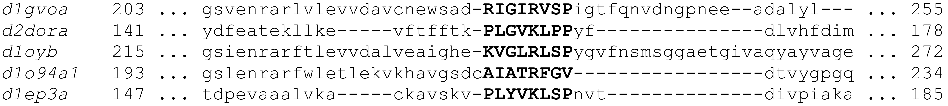
\includegraphics[width=\textwidth]{chapter_1/figures/alignments_a.pdf}
		(a) Higher Accuracy Alignment
	\par\vspace{1em}
		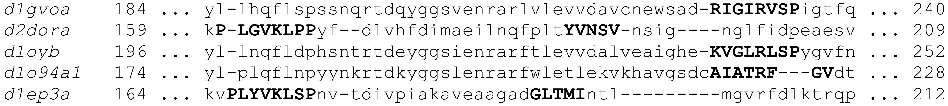
\includegraphics[width=\textwidth]{chapter_1/figures/alignments_b.pdf}
		(b) Lower Accuracy Alignment
	\caption[This part goes into the list of figures]{
		This is the caption that ends up below the figure. 
	}
	\label{fig:alignCompare}
\end{figure}
% !TEX root = ../dissertation.tex

\section{Background}
\label{sec:ch1:background}

Maybe this section should have a table:


\begin{table}	
\centering
\caption[This is what ends up in the list of tables]{
\emph{This is above the table itself}}
\label{table:consistency}
\small
\begin{tabular}{lcccc}
\hline
\hline
\multicolumn{1}{c}{Parameter choice}
  & \multicolumn{4}{c}{Advisor set} \\
\multicolumn{1}{c}{$(\sigma,\,\gamma_I,\,\gamma_E,\,\lambda_I,\,\lambda_E)$}
  & \multicolumn{1}{c}{\scriptsize Default}
  & \multicolumn{1}{c}{\scriptsize Greedy}
  & \multicolumn{1}{c}{\scriptsize Exact}
  & \multicolumn{1}{c}{\scriptsize Oracle} \\
\hline
\\[.5ex]
\multicolumn{1}{c}{$k = 2$} & \multicolumn{4}{l}{} \\
\hline
$\bigl(\Vtml\texttt{200},	50,	17,	41,	40\bigr)$   &	$(2)$ 	&	$(2)$  	&	    	&		\\
$\bigl(\Vtml\texttt{200},	55,	30,	45,	42\bigr)$   &		&	$(2)$	&	$(3)$ 	&	$(1)$	\\
$\bigl(\texttt{BLSUM}\texttt{80},	60,	9,	43,	42\bigr)$   &		&		&	$(2)$	&		\\
$\bigl(\texttt{BLSUM}\texttt{45}, 65, 35, 44, 44\bigr)$ 		  &		&		&	    	&	$(3)$	\\
\hline
\\[.5ex]
\multicolumn{1}{c}{$k = 3$} & \multicolumn{4}{l}{} \\
\hline
$\bigl(\Vtml\texttt{200}, 50, 17, 41, 40\bigr)$	  	&	$(2)$	&	$(2)$	&		&		\\
$\bigl(\Vtml\texttt{200}, 55, 30, 45, 42\bigr)$	 	&		&	$(3)$	&	$(5)$ 	&	$(1)$	\\
$\bigl(\texttt{BLSUM}\texttt{80}, 60, 26, 43, 43\bigr)$ 	&		&	$(2)$	&	$(2)$	&		\\
$\bigl(\Vtml\texttt{200}, 55, 30, 41, 40\bigr)$	 	&		&		&	$(6)$	&		\\
$\bigl(\Vtml\texttt{40}, 45, 29, 40, 39\bigr)$		&		&		&		&	$(7)$	\\
$\bigl(\texttt{BLSUM}\texttt{62}, 65, 16, 44, 42\bigr)$ 	&		&		&		&	$(8)$	\\
\hline
\\[.5ex]
\multicolumn{1}{c}{$k = 4$} & \multicolumn{4}{l}{} \\
\hline
$\bigl(\Vtml\texttt{200}, 50, 17, 41, 40\bigr)$	  	&	$(2)$	&	$(2)$	&		&		\\
$\bigl(\Vtml\texttt{200}, 55, 30, 45, 42\bigr)$	 	&		&	$(3)$	&	$(9)$ 	&	$(6)$	\\
$\bigl(\texttt{BLSUM}\texttt{80}, 60, 26, 43, 43\bigr)$ 	&		&	$(2)$	&		&		\\
$\bigl(\Vtml\texttt{200}, 60, 15, 41, 40\bigr)$	 	&		&	$(1)$	&		&		\\
$\bigl(\Vtml\texttt{200}, 45, 6, 40, 40\bigr)$	 	&		& 		&	$(8)$	 &	$(1)$	\\
$\bigl(\Vtml\texttt{200}, 55, 30, 41, 40\bigr)$	 	&		&		&	$(8)$	&		\\
$\bigl(\texttt{BLSUM}\texttt{80}, 55, 19, 43, 42\bigr)$ 	&		&		&	$(1)$	&		\\
$\bigl(\Vtml\texttt{40}, 45, 29, 40, 39\bigr)$		&		&		&		&	$(4)$	\\
$\bigl(\texttt{BLSUM}\texttt{62}, 65, 35, 44, 42\bigr)$ 	&		&		&		&	$(3)$	\\
\hline
\hline
\end{tabular}
\end{table}


\section{Plan of the dissertation}
This may refer to chapters other than Chapter~\ref{ch:background}

This template was used to produce my dissertation~\citep{D16}, 
and it was passed around by graduate students at the University of Arizona. At this point, I do not think they require a template,
but some may still find it useful. 



% Include the various appendices
%\appendix
%\include{appendix_A}

% Switch the spacing to single-spaced for the references
\renewcommand{\baselinestretch}{1}		% chaning the value
\small\normalsize						% switch size to make the value take

% Create the References list
\bibliographystyle{uabibnat}
\bibliography{dissertation}


\end{document}
